\documentclass[12pt]{article}

%%%%%%%%%%%%%%%%%%%%%%%%%%
%%%  COMMON PACKAGES  %%%%
%%%%%%%%%%%%%%%%%%%%%%%%%%

\usepackage{amsmath}
\usepackage{amssymb}
\usepackage{amsfonts}
\usepackage{graphicx}
\usepackage[utf8]{inputenc}
\usepackage{amsthm}

%%%%%%%%%%%%%%%%%%%%%%%%%%%%%%%%%
%%%  UNUSUAL PACKAGES        %%%%
%%%  Uncomment as necessary. %%%%
%%%%%%%%%%%%%%%%%%%%%%%%%%%%%%%%%

%% MATH AND PHYSICS SYMBOLS
%% ------------------------
\usepackage{slashed}       % \slashed{k}
\usepackage{mathrsfs}      % Weinberg-esque letters
\usepackage{pifont}        % check marks
\usepackage{bbm}           % \mathbbm{1} 
%\usepackage[normalem]{ulem} % for \sout
\usepackage{cancel}

%% CONTENT FORMAT AND DESIGN
%% -------------------------
\usepackage[dvipsnames]{xcolor}
\usepackage{fancyhdr}		% to put preprint number
\usepackage{lipsum}         % block of text 
\usepackage{framed}         % boxed remarks
\usepackage{subcaption}     % subfigures
\usepackage{cite}           % group cites
%\usepackage{tocloft}       % Table of Contents	
\usepackage{xspace}			% spacing after macros
\usepackage{listings}       % code environment	
\lstset{
		basicstyle=\ttfamily\footnotesize,
		breaklines=true,
		backgroundcolor=\color{gray!15!white}}


%% TABLES IN LaTeX
%% ---------------
\usepackage{booktabs}      % professional tables
\usepackage{nicefrac}      % fractions in tables,
\usepackage{multirow}      % multirow elements 
\usepackage{arydshln} 	    % dashed lines in arrays

%% Other Packages and Notes
%% ------------------------
\usepackage[font=small]{caption} % small capt font
\usepackage{float}         % for strict placement e.g. [H]


%% CUSTOM PACKAGES
%% ---------------
\usepackage{tikzfeynman}   % Flip's rules Feynman Diagrams



%%%%%%%%%%%%%%%%%%%%%%%%%%%%%%
%%%  DOCUMENT PROPERTIES  %%%%
%%%%%%%%%%%%%%%%%%%%%%%%%%%%%%
\usepackage[margin=2cm]{geometry}   % margins
\graphicspath{{figures/}}			% figure folder
\numberwithin{equation}{section}    % set equation numbering


%% References in two columns, smaller
%% http://tex.stackexchange.com/questions/20758/bibliography-in-two-columns-section-title-in-one
\usepackage{multicol}
\usepackage{etoolbox}
\usepackage{relsize}
\patchcmd{\thebibliography}
  {\list}
  {\begin{multicols}{2}\smaller\list}
  {}
  {}
\appto{\endthebibliography}{\end{multicols}}


% Change list spacing
% from: http://en.wikibooks.org/wiki/LaTeX/List_Structures#Line_spacing
\let\oldenumerate\enumerate
\renewcommand{\enumerate}{
  \oldenumerate
  \setlength{\itemsep}{1pt}
  \setlength{\parskip}{0pt}
  \setlength{\parsep}{0pt}
}

\let\olditemize\itemize
\renewcommand{\itemize}{
  \olditemize
  \setlength{\itemsep}{1pt}
  \setlength{\parskip}{0pt}
  \setlength{\parsep}{0pt}
}


%%%%%%%%%%%%%%%%%%%%%%%%%%%
%%%  (RE)NEW COMMANDS  %%%%
%%%%%%%%%%%%%%%%%%%%%%%%%%%

%% FOR `NOT SHOUTING' CAPS (e.g. acronyms)
%% ---------------------------------------
\newcommand{\acro}[1]{\textsc{\MakeLowercase{#1}}}    

%% COMMON PHYSICS MACROS
%% ---------------------
\renewcommand{\tilde}{\widetilde}   % tilde over characters
\renewcommand{\vec}[1]{\mathbf{#1}} % vectors are boldface
\newcommand{\dbar}{d\mkern-6mu\mathchar'26}    % for d/2pi
\newcommand{\ket}[1]{\left|#1\right\rangle}    % <#1|
\newcommand{\bra}[1]{\left\langle#1\right|}    % |#1>
\newcommand{\Xmark}{\text{\sffamily X}}        % cross out

%% COMMANDS FOR TEMPORARY COMMENTS
%% -------------------------------
\newcommand{\comment}[2]{\textcolor{red}{[\textbf{#1} #2]}}
\newcommand{\flip}[1]{{
	\color{green!50!black} \footnotesize [\textbf{\textsf{Flip}}: \textsf{#1}]
	}}


%% COMMANDS FOR TOP-MATTER
%% -----------------------
\newcommand{\email}[1]{\href{mailto:#1}{#1}}
\newenvironment{institutions}[1][2em]{\begin{list}{}{\setlength\leftmargin{#1}\setlength\rightmargin{#1}}\item[]}{\end{list}}


%% COMMANDS FOR LATEXDIFF
%% ----------------------
%% see http://bit.ly/1M74uwc
\providecommand{\DIFadd}[1]{{\protect\color{blue}#1}} %DIF PREAMBLE
\providecommand{\DIFdel}[1]{{\protect\color{red}\protect\scriptsize{#1}}}

%% REMARK: use latexdiff option --allow-spaces
%% for \frac, ref: http://bit.ly/1iFlujR


%%%%%%%%%%%%%%%%%%%%%%%%%%%%%%%%%%%%%%%%%%%%%%
%%%  TIKZ COMMANDS FOR EXTERNAL DIAGRAMS  %%%%
%%%  requires -shell-escape               %%%%
%%%  in texpad 1.7: prefs > shell esc sec %%%%
%%%%%%%%%%%%%%%%%%%%%%%%%%%%%%%%%%%%%%%%%%%%%%

%% For exporting tikz figures as into a ./tikz/ subfolder.
%% It is useful if you want pdf versions of the tikz diagrams or
%% if you need to speed up compilation of a large document with
%% many tikz diagrams.

%\write18{} % Careful with this!
%\usetikzlibrary{external}
%\tikzexternalize[prefix=tikz/] % folder for external pdfs


%%%%%%%%%%%%%%%%%%%
%%%  HYPERREF  %%%%
%%%%%%%%%%%%%%%%%%%

%% This package has to be at the end; can lead to conflicts

\usepackage[
	colorlinks=true,
	citecolor=green!50!black,
	linkcolor=NavyBlue!75!black,
	urlcolor=green!50!black,
	hypertexnames=false]{hyperref}


%%%%%%%%%%%%%%%%%%%%%
%%%  TITLE DATA  %%%%
%%%%%%%%%%%%%%%%%%%%%

%% PREPRINT NUMBER USING fancyhdr
%% Don't forget to set \thispagestyle{firststyle}
%% ----------------------------------------------
\renewcommand{\headrulewidth}{0pt} 	% no separator
\setlength{\headheight}{15pt} 		% min to avoid fancyhdr warning
\fancypagestyle{firststyle}{
	\rhead{\footnotesize%
%	\texttt{UCI-TR-2016-XX}\\ %% Uncomment for additional preprint #s
	\texttt{UCR-PHYS-165-W2018-B}%
	}}

%% TOC overwrites fancyhdr, here's a fix
%% http://tex.stackexchange.com/questions/167828/difficult-with-fancyhdr-and-table-of-contents
\usepackage{etoc}
\renewcommand{\etocaftertitlehook}{\pagestyle{plain}}
\renewcommand{\etocaftertochook}{\thispagestyle{firststyle}}



\begin{document}

%\thispagestyle{empty}		% default if no preprint #
\thispagestyle{firststyle} 	% to include preprint

\begin{center}

    {\huge \bf P165: Introduction to Particle Physics}{\Large \bf \\ Monte Carlo Notes}

    \vskip .7cm

%% SINGLE AUTHOR FORMAT
%% --------------------
	Prof.~\textbf{Flip Tanedo} %\\
	(\texttt{\footnotesize \email{flip.tanedo@ucr.edu}})

	\vspace{-1em}
    \begin{institutions}[2.25cm]
    \footnotesize
    {\it 
	    Department of Physics \& Astronomy, 
	    University of  California, Riverside, 
	    {CA} 92521	    
	    }    
    \end{institutions}


\end{center}




%%%%%%%%%%%%%%%%%%%%%
%%%  ABSTRACT    %%%%
%%%%%%%%%%%%%%%%%%%%%

\begin{abstract}
\noindent 
These are course notes for Physics 165 focusing on using \texttt{MadGraph}. 
\\
\textbf{These notes are in progress}. Last update: \today
\end{abstract}



\small
\setcounter{tocdepth}{2}
\tableofcontents
\normalsize
%\clearpage


%%%%%%%%%%%%%%%%%%%%%
%%%  THE MEAT    %%%%
%%%%%%%%%%%%%%%%%%%%%

%% Use \input if you have separate files.
%% \include is `smarter' (creates separate aux files
%% for each tex file) and hence more efficient, 
%% but it automatically puts a page break
%% between included files. Input doesn't do this.


\section{The MadGraph 5 Web Interface}

The \texttt{MadGraph} development team maintains a limited web version of \texttt{MadGraph} 5 at the following address: \url{http://madgraph.phys.ucl.ac.be}

It should look something like this:

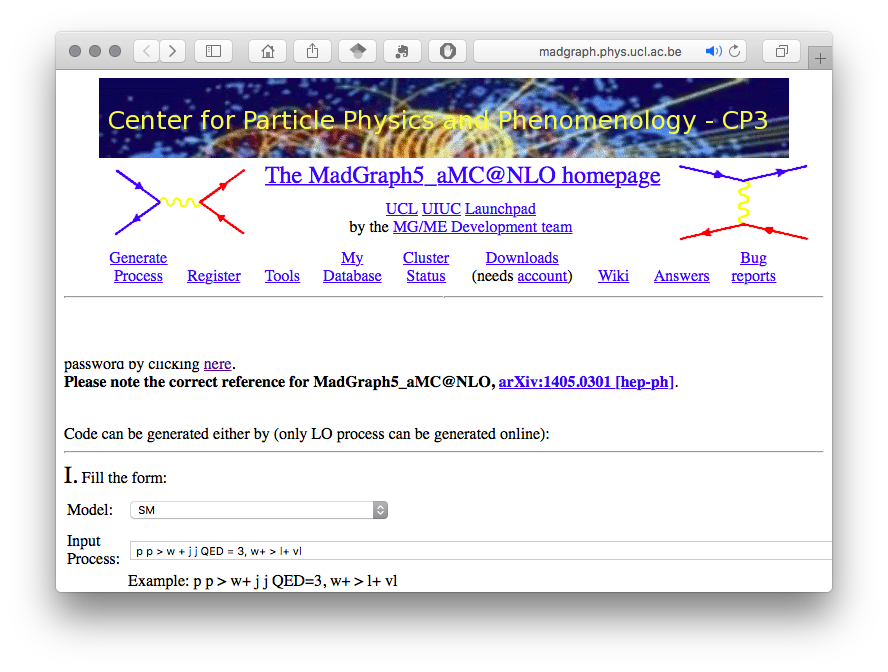
\includegraphics[width=.8\textwidth]{MG5website.png}

\subsection{Instructions}
\begin{enumerate}
	\item Click on the \textbf{Register} link.
	\item Fill out the form; use your \acro{UCR} e-mail address and set your institution as \acro{UCR}.
	\item You will receive an e-mail from \texttt{madgraph@madgraph.cism.ucl.ac.be} with your username and password. Save this information.
\end{enumerate}


\section{Installing MadGraph 5}




\section*{Acknowledgements}


%
\textsc{p.t.}\ thanks 
\emph{your name here}
for useful comments and discussions. 
%
\textsc{p.t.} thanks the Aspen Center for Physics (NSF grant \#1066293) for its hospitality during a period where part of this work was completed.

%% Appendices
% \appendix


%% Bibliography
\bibliographystyle{utphys} 	% arXiv hyperlinks
% \bibliography{bib title without .bib}


\end{document}